\documentclass[12pt]{article}
\usepackage[margin=1in]{geometry}
\usepackage{amsmath,amssymb,amsthm,booktabs,graphicx,natbib,microtype,array}
\newtheorem{theorem}{Theorem}
\newtheorem{corollary}[theorem]{Corollary}
\newtheorem{proposition}[theorem]{Proposition}
\newtheorem{remark}[theorem]{Remark}
\title{Delayed Start and Isolation of Superunit Birth Events\\\large Finite-Prefix Invariance versus Recurrent Viability Obstructions}
\author{Prime Dynamics Theory Program}
\date{July 2026}

\begin{document}
\maketitle

\begin{abstract}
RH-144 proves that two coarse finite chains have empty controlled viability
kernels because every candidate control has a zero-state floor above one.
We determine what this means asymptotically.  Finite deletion does not change
\[
 \limsup y_n,
 \qquad \liminf a_n,
 \qquad
 \liminf (1-\sqrt{y_n})_+^4a_n.
\]
Hence a proof may start after a finite exceptional prefix, provided a reset
enters a future controlled-invariant tube.  Conversely, if
\[
 m_n=\inf_{c\in\mathcal C_n}F_{n,c}(0)\geq1
\]
for infinitely many $n$, then every nonnegative controlled trajectory has
$\limsup y_n\geq1$.  A recurrent superunit floor is therefore a genuine
asymptotic obstruction; a finite one is not.

The finite archive contains exactly two superunit birth coefficients, both
at the left $\sigma=0.08$ anchor for thresholds $10^{-8}$ and $10^{-6}$.
Their full candidate-family minimum floor is $9.535>1$, and both backward
kernels are empty.  Nevertheless the cofinal anchor suffix beginning at
$\sigma=0.04$ has 18/18 forward-safe and outward-positive chains.  Its
minimum terminal directional floor exceeds $1.5\times10^{-10}$; at the two
finest anchors the minimum exceeds $9.7\times10^{-4}$.  This rigorously
isolates the known failures as finite-prefix events.  It does not prove that
no analogous birth occurs at an untested future level.
\end{abstract}

\section{Finite failures and asymptotic statements}
The RH-139 frontier is eventual: it asks for $\limsup y_n<1$ and
$\liminf a_n>0$.  Such conditions deliberately ignore finitely many initial
indices.  A finite envelope failure can invalidate a certificate that begins
at level zero while leaving an eventual theorem logically possible.

This observation is not permission to erase an inconvenient point from one
continuous trajectory.  A delayed start must specify a later state enclosure
or reset and prove the future recurrence from there.  RH-144 supplies the
right language: the reset state must enter a positive backward/block kernel
\citep{Aubin1991}.

\section{Cofinal invariance and delayed support}
We record the elementary but essential theorem explicitly.

\begin{theorem}[Finite-prefix invariance]\label{thm:prefix}
For any real sequence $z_n$ and integer $N$,
\[
 \limsup_{n\to\infty}z_n=\limsup_{n\to\infty}z_{n+N},
 \qquad
 \liminf_{n\to\infty}z_n=\liminf_{n\to\infty}z_{n+N}.
\]
Consequently the RH-139 hypotheses and directional lower are unchanged by
deleting a finite prefix.
\end{theorem}
\begin{proof}
The supremum and infimum of a tail are unchanged after removing finitely many
terms once the tail index passes those terms.  Taking limits proves both
identities.  Apply them to $y_n$, $a_n$, and the directional candidate.
\end{proof}

\begin{corollary}[Delayed-start support]\label{cor:start}
Suppose that at some level $N$ a validated reset gives $y_N\leq r$, every
future controlled block preserves a tube with partial-block upper
$\bar y<1$, and $\liminf_{n\geq N}a_n\geq a_*>0$.  Then
\[
 \liminf_{n\to\infty}B_n
 \geq(1-\sqrt{\bar y})^4a_*>0,
\]
regardless of the finite prefix before $N$.
\end{corollary}
\begin{proof}
The block policy gives the tail limsup bound from $N$ onward.  Apply the
RH-139 support theorem to the shifted sequence and then
Theorem~\ref{thm:prefix}.
\end{proof}

\section{The recurrent-floor obstruction}
Finite deletion has a sharp opposite.

\begin{theorem}[Infinitely recurrent superunit floors]\label{thm:recurrent}
Let every controlled envelope be increasing on $[0,\infty)$ and define
\[
 m_n=\inf_{c\in\mathcal C_n}F_{n,c}(0).
\]
If $m_n\geq1$ for infinitely many $n$, then every nonnegative controlled
trajectory obeys $\limsup y_n\geq1$.  In particular the RH-139 tail packet
is impossible for that control family.
\end{theorem}
\begin{proof}
At every such index and for every control,
$y_{n+1}=F_{n,c_n}(y_n)\geq F_{n,c_n}(0)\geq m_n\geq1$.
This occurs infinitely often, so the upper limit is at least one.
\end{proof}

The theorem is architecture relative: enlarging the control family can lower
$m_n$.  Within a fixed family it is exact.  It also shows why an all-level
proof must exclude recurrent bad births, not merely show that their density
tends to zero.

\section{Finite suffix audit}
The RH-137 archive has 330 transitions.  Exactly two selected birth
coefficients exceed one:
\[
 q=9.405889994899066.
\]
Both occur on the left $\sigma=0.08$ anchor, at the final transition, for
thresholds $10^{-8}$ and $10^{-6}$.  RH-144 strengthens this observation by
minimizing over the entire gauge family: the least zero-state floor is still
$9.5352>1$, and the predecessor kernel is empty in both cases.

We order the five finite anchors toward finer scale and delete successively
larger prefixes.  The same audit is applied to the forward RH-137 chains and
the outward RH-138 directional composition.

\begin{table}[t]
\centering
\scriptsize
\begin{tabular}{ccccc}
\toprule
start cutoff & suffix chains & forward safe & outward positive & minimum positive terminal floor\\
\midrule
$0.16$ & $30$ & $28$ & $28$ & $1.04\times10^{-10}$\\
$0.08$ & $24$ & $22$ & $22$ & $1.55\times10^{-10}$\\
$0.04$ & $18$ & $18$ & $18$ & $1.55\times10^{-10}$\\
$0.02$ & $12$ & $12$ & $12$ & $9.76\times10^{-4}$\\
$0.01$ & $6$ & $6$ & $6$ & $2.14\times10^{-3}$\\
\bottomrule
\end{tabular}
\caption{Cofinal finite-anchor suffixes.}
\label{tab:suffix}
\end{table}

Thus $\sigma=0.04$ is the first completely clean archived suffix.  The
coarser $\sigma=0.16$ chains happen to be safe, but a cofinal start after the
bad $0.08$ anchor necessarily discards them as part of the finite prefix.

\begin{figure}[t]
\centering
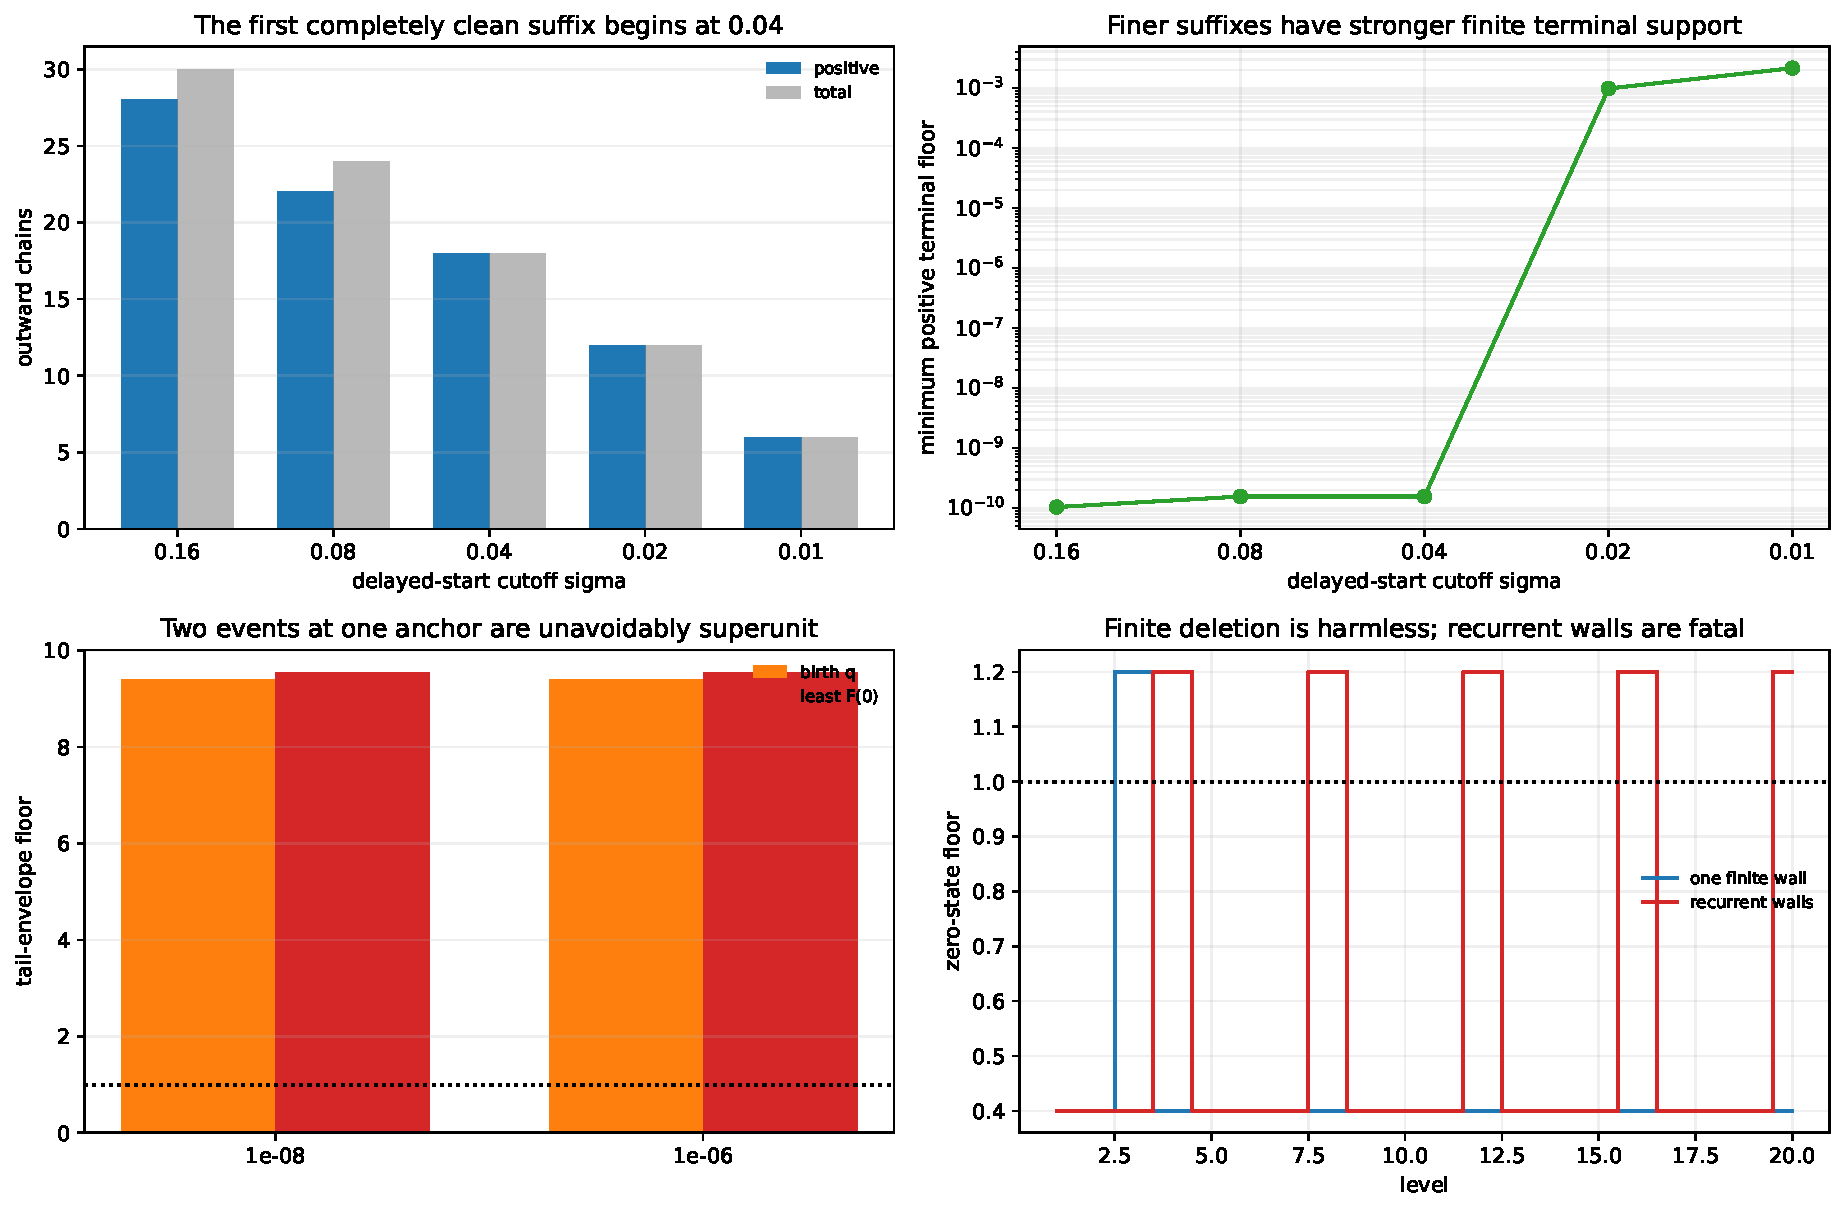
\includegraphics[width=\textwidth]{figures/delayed_start_birth_isolation.pdf}
\caption{Suffix classifications and floors, the two isolated superunit
events, and the finite-versus-recurrent distinction.}
\label{fig:audit}
\end{figure}

\section{Consequence and claim boundary}
The known coarse failures no longer need to be ``repaired'' in an eventual
theorem.  A valid route may start after them.  Its remaining obligations are
precise: produce a validated reset at the delayed start, prove a common future
block kernel and partial safety gap, and prove the normalized-base liminf.

The clean 18-chain suffix is finite evidence for this strategy, not proof
that every future level is clean.  We have not excluded recurrent superunit
births analytically, constructed an all-level delayed reset, proved a uniform
tail gap or base liminf, established Stage A, constructed a Hilbert--Polya
operator, identified zeta zeros, or proved the Riemann Hypothesis.

\bibliographystyle{plainnat}
\bibliography{references}
\end{document}
